\section{Experimental Evaluation}
\begin{figure*}[ht]

    \begin{subfigure}[b]{0.25\linewidth}
        \centering
        %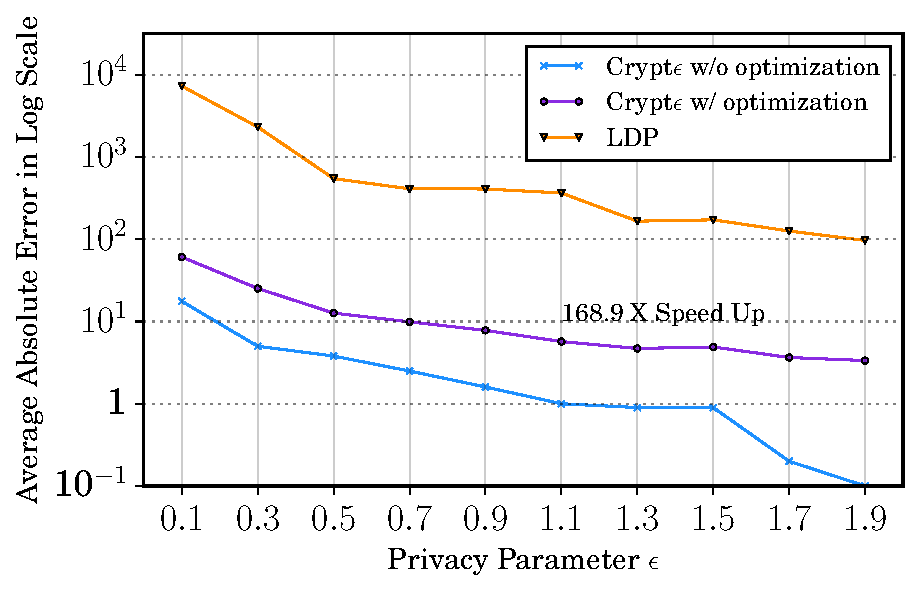
\includegraphics[width=5cm,height=3.1cm]{t1.pdf}
         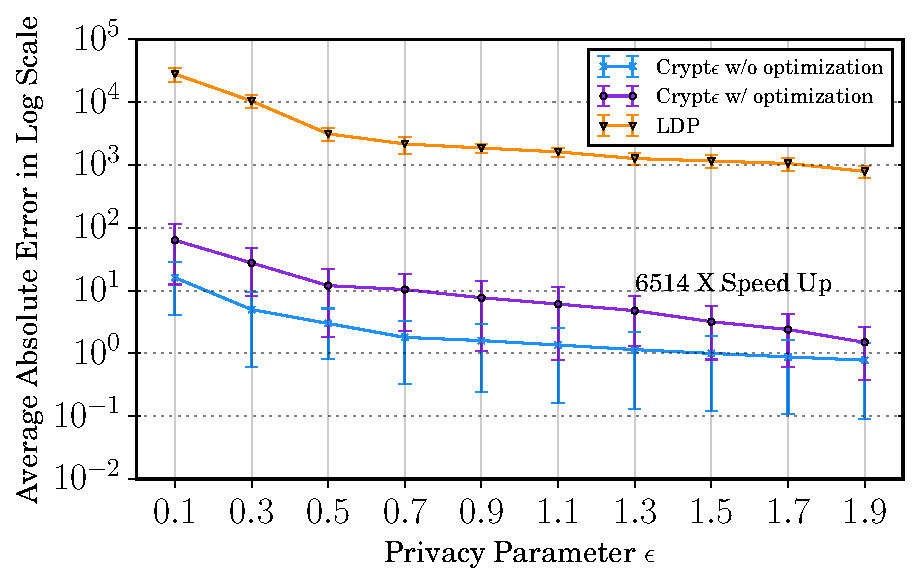
\includegraphics[width=1\linewidth]{t1_final.pdf}
        \caption{ Accuracy Analysis of Program A}
        \label{fig:P1}
    \end{subfigure}%%
    \begin{subfigure}[b]{0.25\linewidth}
    \centering 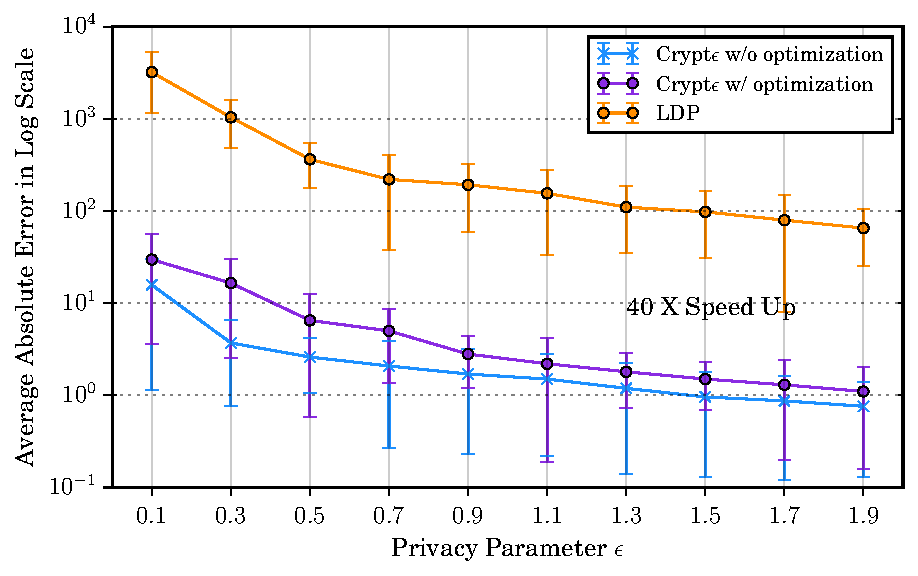
\includegraphics[width=1\linewidth]{t5_final.pdf}
        \caption{Accuracy Analysis Program B}
        \label{fig:mouse}\end{subfigure}%%
    \begin{subfigure}[b]{0.25\linewidth}
    \centering    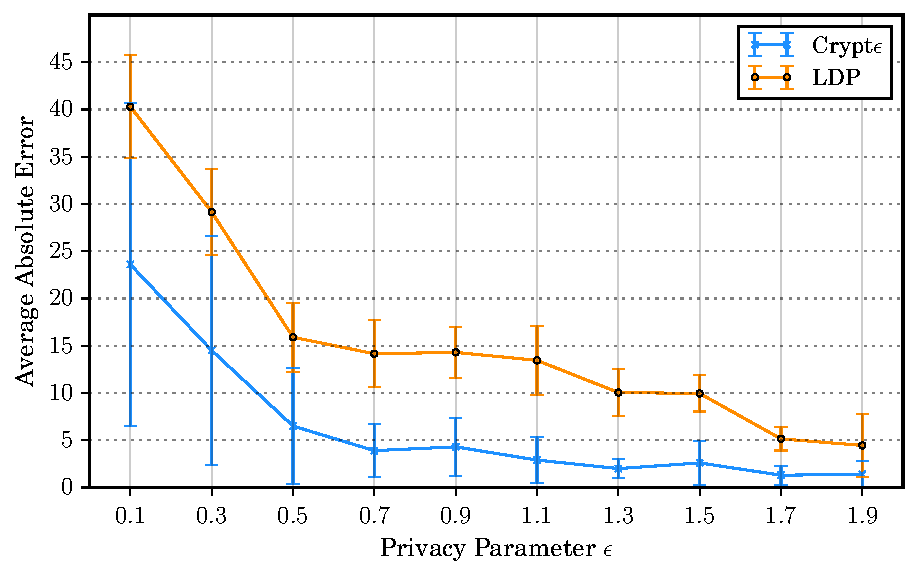
\includegraphics[width=1\linewidth]{t7_final.pdf}
        \caption{Accuracy Analysis of Program C}
        \label{fig:P5}\end{subfigure}%%
      \begin{subfigure}[b]{0.25\linewidth}
    \centering    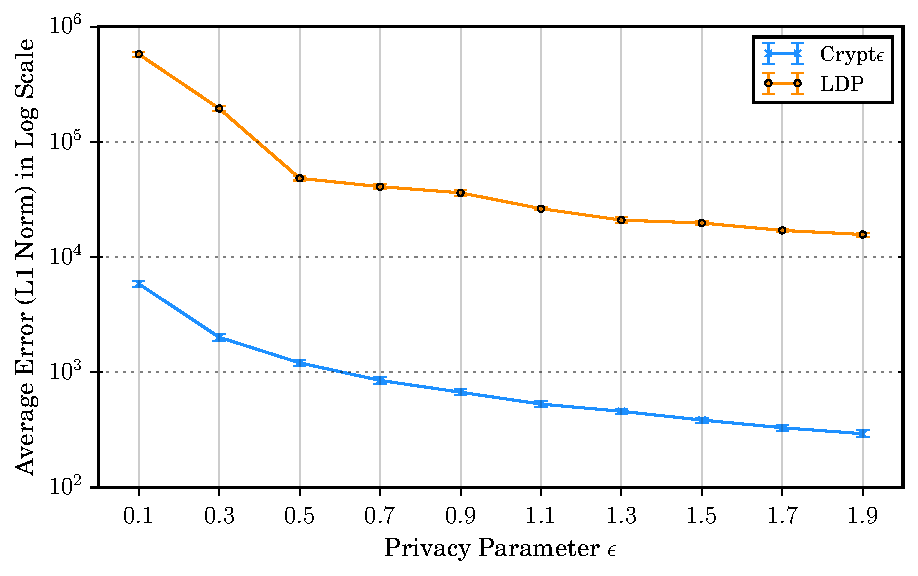
\includegraphics[width=1\linewidth]{t3_final.pdf}
        \caption{Accuracy Analysis of Program D}
        \label{fig:P7}
    \end{subfigure}%%
    
    \begin{subfigure}[b]{0.25\linewidth}
     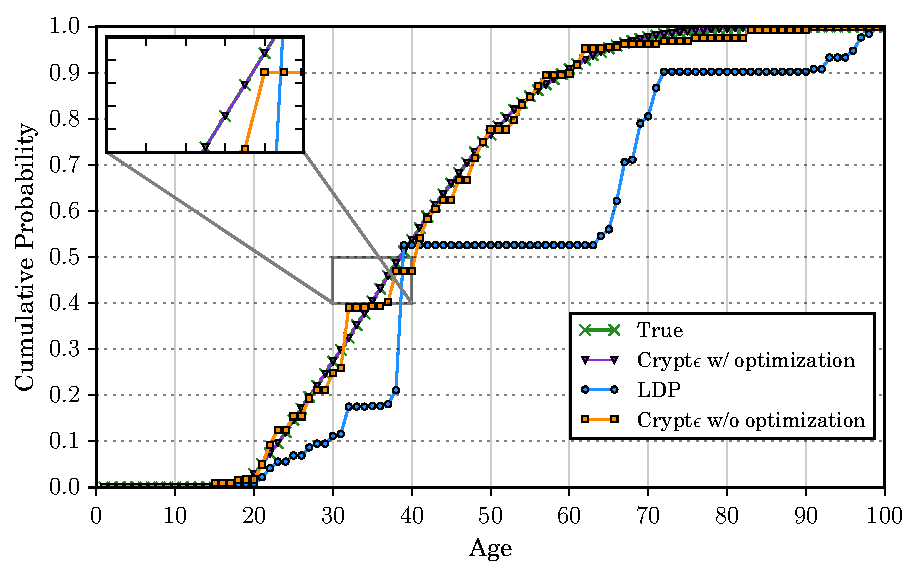
\includegraphics[width=1\linewidth]{cdf_final.pdf}
        \caption{DP Range Tree Evaluation}
        %\label{rangetree}
        \end{subfigure}
        \begin{subfigure}[b]{0.25\linewidth}
     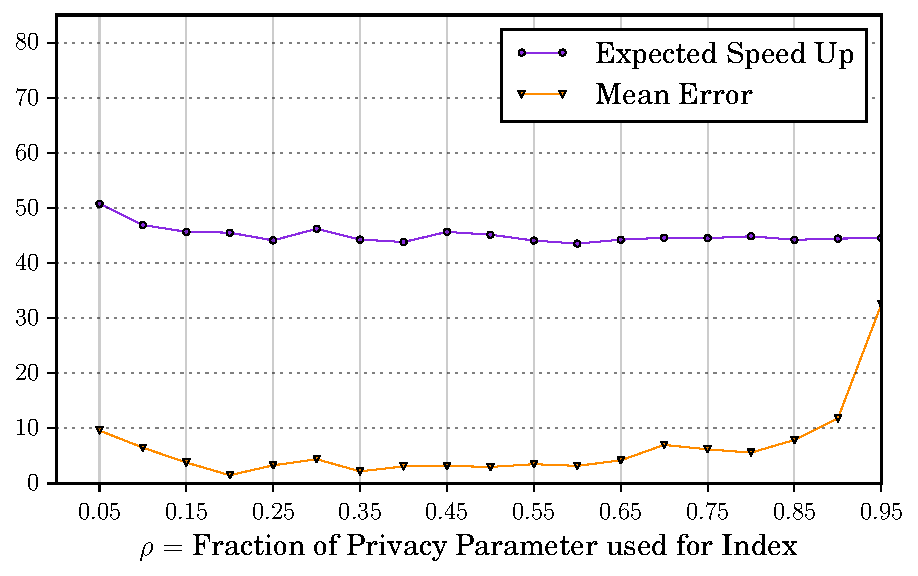
\includegraphics[width=1\linewidth]{index_final.pdf}
        \caption{Privacy Budget Analysis for DP Index}
        \label{Index}
    \end{subfigure}
    \begin{subfigure}[b]{0.25\linewidth}
     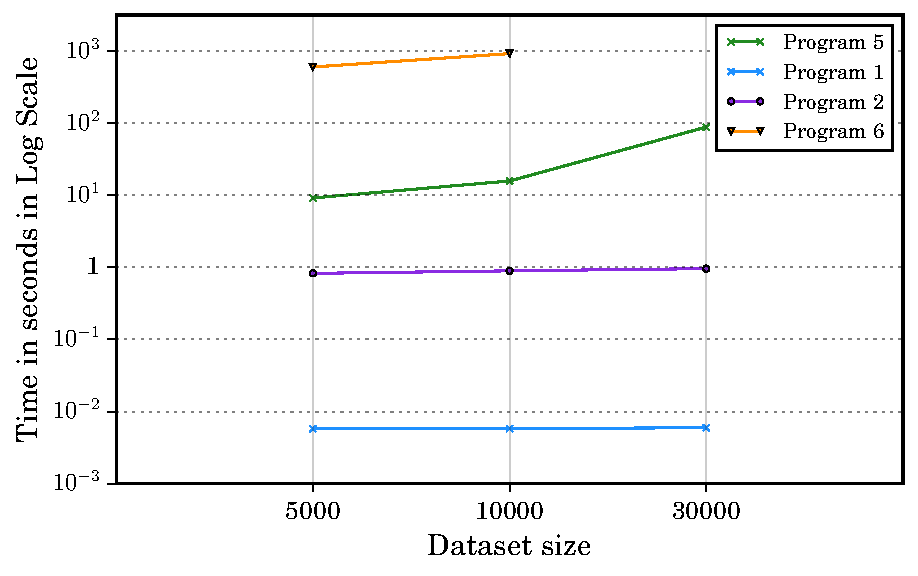
\includegraphics[width=1\linewidth]{scalet.pdf}
        \caption{\system Program Scalability}
        \label{Scale}
    \end{subfigure}
   \caption{Empirical Evaluation of Crypt$\epsilon$ Programs}
\end{figure*}
In this section we experimentally evaluate  Crypt$\epsilon$ to assess its practical utility  based on two parameters, the accuracy and the performance of the Crypt$\epsilon$ programs. Specifically \\(1) Does Crypt$\epsilon$ programs have constant error bounds depending only on the privacy parameter $\epsilon$  which is at least $O(\sqrt{m})$ times lower than that for the corresponding state-of-the-art LDP implementation?\\(2) Does the proposed DP- optimizations provide substantial performance improvement over the base case Crypt$\epsilon$ implementation? \\ (3) Is the program execution timings for optimized Crypt$\epsilon$ practical?\\
\eat{\textbf{Evaluation Highlights:}
As seen in figures the depend only on the orivacy parameter and hence are . Moreover The optimizations with a spped up of and respectively
The with respectively. Finally \system programs run pretty fast.  on a dataset of 32561 records.  Whie progra finish ij just a few seconds an while minutes. As seen in figures the depend only on the orivacy parameter and hence are . Moreover The optimizations with a spped up of and respectively
The with respectively. Finally \system programs run pretty fast.  on a dataset of 32561 records.  Whie progra finish ij just a few seconds an while minutes. As seen in figures the depend only on the orivacy parameter and hence are . Moreover The optimizations with a spped up of and respectively
The with respectively. Finally \system programs run pretty fast.  on a dataset of 32561 records.  Whie progra finish ij just a few seconds an while minutes. }
%The accuracy analysis in show case that for the are at least smaller . From table we see that can provide to while  speed up in execution time. Moreover 
%%That the performnace arefaesble with the just taking while . the longest is 
%We elaborate each of the above three obseravations in three separate sections as followed.
\subsection{Methodology} 
\textbf{Programs:}
To answer the aforementioned questions we ran the experiments on 4 of the Crypt$\epsilon$ programs previously outlined in Table 3, namely P1,P3,P5 and P7. In this section we rename P1,P5,P7 and P3 as Program A, Program B, Program C and Program D respectively.  Each program is compared with the corresponding state-of-the-art \textsf{LDP} implementations. Additional experimental results for programs P2,P4 and P6 from Table 3 are presented in Appendix.% We rename the examples 5.1,5.2,5.3,5.4,5.6 and 5.7 as P1,P2,P6,. The reason behind this grouping is to arrange the programs in their increasing order of complexity.  %\begin{itemize}\item \textbf{Program 1} - Count the number of records having age in range $[50,60]$ \\\textbf{\textsf{LDP} Competitor} - Frequency oracle of \cite{LDP1} constructed over attribute $Age$. \item \textbf{Program 2} - Report the top 5 most frequent age values. \\\textbf{\textsf{LDP} Competitor} - Frequency oracle of \cite{LDP1} constructed over attribute $Age$.  \item \textbf{Program 3 }- Report the marginal on attributes $Age$ and $Gender$. \\\textbf{\textsf{LDP} Competitor }- Frequency oracle of \cite{LDP1} constructed over attribute $Age \times Gender$. \item \textbf{Program 4 }- Report the marginal on attributes $Age$ and $Gender$ with $NativeCountry=Mexico$\\\textbf{\textsf{LDP} Competitor }- Frequency oracle of \cite{LDP1} constructed over attribute $Age\times Gender \times NativeCountry$. \item \textbf{Program 5 }- Count the number of natively Mexican male employees of age 30.\\\textbf{\textsf{LDP} Competitor }- Frequency oracle of \cite{LDP1} constructed over attribute $Age\times Gender \times NativeCountry$. \item \textbf{Program 6 }- Count the number of distinct age values for male employees. \\\textbf{\textsf{LDP} Competitor }-Frequency oracle of \cite{LDP1} constructed over attribute $Age\times Gender$.% and reports the number of non-zero counts after suitable adjustment for thresholding. 
%\item \textbf{Program 7 }- Count the number of age values with at least 10 records. \\\textbf{\textsf{LDP} Competitor }- Frequency oracle of \cite{LDP1} constructed over attribute $Age$. \end{itemize}
\\\textbf{Datasets:}
We ran our experiments on the Adult dataset from the UCI repository \cite{UCI}  which has been extracted from the 1994 census data. The dataset is of size $32,651$ and the experiment numbers are reported as the mean value after 10 repetitions.
\\\textbf{Metrics:}
\\\textbf{\textit{Accuracy:}} For accuracy the following metrics are used
\\$\bullet$ Programs A, B and C use absolute error $ =|C-\hat{C}|$ where $C$ is the true count and $\hat{C}$ is the noisy output.\\ $\bullet$ Programs D uses the $L1-Norm$ error metric given  by $Error=\sum_{i}|C[i]-\hat{C}[i]|, i \in [|C|]$.\\
\textbf{\textit{Performance:}} For measuring performance we report the total execution time in seconds for each program.


%uses the error measure given by the fraction of age values returned in the top 5 that have value less than $ct_5-\alpha$  where  $ct_5$ is the count of the $5^{th}$ largest value and $\alpha=\frac{1}{\epsilon}\log\frac{1}{\delta}$ is a slack parameter. The slack parameter is required because with probability $1-\delta$ no differentially private algorithm can distinguish between any two counts that differ by less than $\alpha$. We use $\delta=0.05$ for our experiment. \item Programs 3, 4 and 5 \end{itemize}



\subsection{Evaluation of Goal 1}
\stitle{Accuracy of base case \system implementations}
The first observation with respect to accuracy, is that the error for a single frequency counting program for the base case Crypt$\epsilon$ implementation is of the order $O(\frac{1}{\epsilon})$. In fact quantitatively it is close to $\frac{2}{\epsilon}$. This conforms to our expectation as we add two instances of Laplace noise at the \textsf{AS} and the \textsf{CSP} and s.t.d of $Lap(\frac{1}{\epsilon})$ is given by $\frac{1}{\epsilon}$. For e.g., in Figure 2a we observe that for Program A, mean error of base case \system is $16.10$ for $\epsilon=0.1$ and $0.78$ for $\epsilon=1.9$. Similarly for Program B, Figure 2b shows that  $\epsilon=0.1$ results in a mean error of $15.8$ for base case \system while for $\epsilon=1.9$ we get a mean error of $0.76$. Figure 2d shows that  for Program D, the  error for Crypt$\epsilon$ is approximately $200\cdot 2 \times $ larger than that for Programs A and B. For e.g., mean error for Program B is $5862.4$ and $292.9$ for $\epsilon=0.1$ and $\epsilon=1.9$ respectively. It is so because, the attribute $Age$ has domain size $100$ while attribute $Gender$ is of size $2$. Hence $Age\times Gender$ is of domain size $200$. the additional factor of $2$ comes from the fact that, Program D uses the $\textsf{GroupBy}^*$ primitive which is 2-stable.  
 \par 
\stitle{Accuracy of \textsf{LDP} implementation } For a single noisy count, the error corresponding to that of the $\textsf{LDP}$ implementations is of the order $O(\frac{\sqrt{m}}{\epsilon})$. For Program A, we observe in Figure 2a that the error values are at least $1000 \approx \frac{11}{2}\cdot \sqrt{m}=  \frac{11}{2}\cdot \sqrt{323561}$ times worse. This observation is intuitive as for answering Program A we need to read $11$ noisy counts from the frequency oracle (for the range [50,60]) and the factor of $\frac{1}{2}$ comes from the fact that the errors in Crypt$\epsilon$ are roughly $\frac{2}{\epsilon}$. For e.g., the error for $\textsf{LDP}$ is $1747 \times$  higher than that of Crypt$\epsilon$ for $\epsilon=0.1$. As expected, Program B has at least $90 \approx \frac{\sqrt{32561}}{2}$ times worse errors for the \textsf{LDP} implementation as is seen in Figure 2b. For e.g., for $\epsilon=0.1$ the error for $\textsf{LDP}$ is $200\times $ worse than the base case \system implementation. Moreover we observe that the \textsf{LDP} implementation errors for Progarm B are roughly $\frac{1}{11}\times$ that of the corresponding errors for Program A. It is so because Program B outputs a single noisy count only. Similarly, for Program D, we observe in Figure 2d that the error values of the $\textsf{LDP}$ implementation is around $\frac{\sqrt{m}}{4}=45 $ times higher than that of base case Crypt$\epsilon$. There is an extra $\frac{1}{2}$ factor since  the corresponding \system program is $2-$ stable. For e.g., $\epsilon=0.1$ results in almost $98 \times$ higher error for the \textsf{LDP} implementation as compared to that of the base case \system implementation. As expected, the mean errors for the \textsf{LDP} implementation are around $18 = 200/11$ times that of the corresponding values for Program A and $200\times$ that of the corresponding values for Program B.
\par
Recall Program C outputs the number of age values with at least 100 records. Thus Program C does not directly report counts of records in the database but some statistic based on the counts. Even here we observe that the accuracy of Crypt$\epsilon$ is significantly higher than that of the corresponding \textsf{LDP} implementations. For e.g., Figure 2c shows that for $\epsilon=0.1$ the error for Crypt$\epsilon$ is $23.6$ while that for the \textsf{LDP} implementation is $40.3$. \\
\stitle{Accuracy of optimized \system implementation}\\
\stitle{DP Range Tree }- From the perspective of execution time, Program A can benefit from a range tree constructed over attribute $Age$.  However, from Figure 2a, we observe that the accuracy of the range tree based Crypt$\epsilon$ implementation is slightly poorer (at most 6 $\times$ worse)  as compared to that of the base case. For e.g., for $\epsilon=0.1$, the mean error for the optimized implementation is $63.5$ while that for the base case is $16.1$. This is so because the sensitivity of the range tree is $\log k$ where $k$ is the number of leaves (100 in this case) and a range query can take up to $2 \log k$ nodes for answering. Thus for a single query, the base case implementation will give better accuracy results. The accuracy gain for range trees kicks in for answering multiple range queries as showcased in Figure 2e.  For this experiment, we construct the c.d.f over the attribute $Age$ by first executing 100 range queries, where the $i$-th query outputs the noisy count for age values in $[1,i], i \in [100]$. This is followed by a isotonic regression post-processing to get a proper c.d.f. We use a total privacy budget of $\epsilon=1$ for all the 100 queries. From a visual analysis of the plots in Figure 2e, we observe that the plots for the true c.d.f and the one obtained from optimized \system are almost indistinguishable. In fact the mean L1-Norm error of the c.d.f for the optimized \system is just $0.0045$. Although the plot for the unoptimized implementation \system captures the overall shape of the c.d.f correctly, it shows slight aberrations in some points and has a mean L1-Norm error of $1.211$. On the other hand, the c.d.f obtained from the \textsf{LDP} implementation is way off and results in a mean L1-Norm error of $12.93$.  \\
\stitle{DP Index}-Program B can be optimized by constructing a DP index over the attribute $nativeCountry$. For our experiments, we use $20\%$ of the total privacy budget towards constructing the index, the remaining $80\%$ is reserved for the rest of the program execution. The rational behind selecting the value $20\%$ will be discussed in the following section. From Figure 2b we observe that the accuracy of the optimized implementation of \system is slightly lower than that of the base case implementation. It is so because consider a program trying to compute the number of records satisfying the Boolean condition $\phi= (A==v)$; now the noisy index constructed over attribute $A$ might miss some of the records having value $v$ for the attribute $A$, thereby introducing additional errors. 
However, as seen in Figure 2b, the increase in error is only $2\times$ at most and hence the optimized implementation still gives constant error bounds (since the noise added to the index is independent of the number of records and depends only on the privacy parameter and the total number of partitions/bins).

The other two implementation based optimizations namely pre-computation and off-line generation, work purely on the encrypted data and have no effect whatsoever on the accuracy of the program outputs. 
\subsection{Evaluation of Goal 2}
 \eat{\begin{table}[ht]
\caption{Execution Time Analysis for Crypt$\epsilon$ Programs}
\small
\centering
\begin{tabular}{c  c c c c c}
\toprule
Program &  \multicolumn{3}{c}{Base} & \multicolumn{2}{c}{Optimized} \\ 
 & AS &  CSP & Total & Total & Speed up  \\ &(s)&(s)&(s)&(s)&$\times$\\ % inserts table %heading
\midrule
1 & 0.49& 0.0027& 0.4927 & 0.0029 & 168.9 \\
2 &  6.12 & 0.3  &6.42 & 0.89 & 7.2\\ %197 the communication rounds
3&  3859.52 & 3661.29 & 7520.81&N/A&N/A \\4  &7765.16&3624.05&11389.21& 910.96 & 12.5 \\5&18.56&16.7&35.26&3.49 & 10.1 \\6&1910.01&571.11&2481.12&429.92 & 5.77\\7&6.35 & 1393.89 & 1400.24 &  N/A & N/A \\ [1ex]
\bottomrule
\end{tabular}
\label{c}
\end{table}}


\begin{table}
\caption{Execution Time Analysis for Crypt$\epsilon$ Programs}
\centering
\scalebox{0.8}{
\begin{tabular}{|c c|c|c|c|c|}
\hline
\multicolumn{2}{|c}{\textbf{Time in (s)}}   & \multicolumn{4}{|c|}{\textbf{Program}}\\
\cline{3-6}&&\textbf{A} & \bf{B} & \bf{C} &\bf{D}  \\ 
\hline \hline
\multirow{3}{*}{\textbf{Base}}& \multicolumn{1}{|c|}{\textsf{AS}} & 18.89 & 650.78& 101792.79 & 3859.53 \\
\cline{2-6}& \multicolumn{1}{|c|}{\textsf{CSP}} & 0.0027 & 550.34 & 78131.21 & 1137.68 \\\cline{2-6}
& \multicolumn{1}{|c|}{Total} & 18.8927 & 1201.12 & 179924 &  4997.21 \\\hline
%\multirow{4}{*}{\textbf{Optimized}}& \multicolumn{1}{|c|}{\textsf{AS}} & .0004 &16.21 &250.17  &\\ \cline{2-6}& \multicolumn{1}{|c|}{\textsf{CSP}} & .0027 &13.92 &0.54 &\\
\multirow{2}{*}{\textbf{Optimized}}& \multicolumn{1}{|c|}{Total} & 0.0031 & 30.13 & 250.71 &  \\
\cline{2-6}& \multicolumn{1}{|c|}{Speed Up $\times$} &6514.7 & 40 &   717.6 &
\\ [1ex]
\hline
\end{tabular}}
\label{c}
\end{table}
\textbf{DP Range Tree}
 For Program A we see that the total time taken for execution for the base case Crypt$\epsilon$ implementation is about 19 seconds while using the range tree optimization we get a $6514\times$ speed up in timings. It is so because the time required by the \textsf{AS} in the optimized implementation becomes almost negligible because it simply needs to do a memory fetch to read off the answer from the pre-computed range tree instead of computing it from the entire encrypted database. %The time for the \textsf{CSP} remains the same in both the cases, it is the decryption cost. For Program 2, we observe a $7\times$ performance improvement with the range tree optimization. Again, the reason is even in this case the \textsf{AS} can simply read off the leaf nodes of the range tree instead of computing their counts from the database. 
\\\textbf{DP Index}- For Program B, we observe that the base case implementation takes around $20$ minutes to run. However  a DP index over the attribute $NativeCountry$  reduces the execution time to about $2s$ only  giving us a $40\times $ speedup. It is so because, only about 2\% of the data records satisfy $NativeCountry$=Mexico. Thus the index reduces the number of records to be considered for the program execution drastically thereby resulting in a huge performance boost. %The 10 drop is due to the 
Let $\rho$ represent the fraction of the privay parameter used towards constructing the DP index. As mentioned before, $\rho=0.2$ in this experimental setup.  In Figure 2f we study how the expected speed up in execution time and the accuracy of the final result vary as a function of $\rho$ for Program B for a total privacy parameter of $\epsilon=1$. We measure the expected speed up as $\frac{\text{Total dataset size=32561}}{\text{\# of records to be considered as indicated by the DP index}}$. From Figure 2f we observe that the error reduces till $\rho=0.2$ and stabilises until $\rho=0.65$ after which it starts rising again. This rise in error is because, as we keep increasing $\rho$, the amount of privacy parameter left for the measurement primitive keeps decreasing and after a certain point ($\rho=0.65$ in our experimental setup), starts dominating the total error. Also we observe that at about $\rho=0.2$, the index is able to approximately identify the correct set of records and hence increasing $\rho$ further does not affect the speed up or its contribution to the total error by much. Hence we choose $\rho=0.2$ for our experiments. A formal accuracy vs speed up trade-off analysis would be very helpful in this regard and is part of our future work.
 \\\textbf{Pre-computation}- For Program D the unoptimized execution time on the dataset of $32561$ records is around 2 days. This is so because the $\textsf{CrossProduct}$ primitive used in the program needs to perform $200\cdot 32561$ $labMult()$ operations which is very time consuming. Hence from Table 4 we see that, pre-computing the 2-dimensional attribute over $Age$ and $Gender$ is a very useful optimization as now the execution reduces to just about 4 minutes giving us a $717.6\times$ speed up. \\ %The un-optimized implementation for  Program D takes . It is because of the \textsf{CrossProduct} Primitiev because ot needs to compute . Pre-computaion f thsi saves a lot of time and cuts down the executioj tiem by.
\textbf{Off-line Processing}
The most costliest primitive for Program C is the specifically since the \textsf{CSP} has to generate for the one-hotcodings. In the base case this takes about . But with the off-line geneates then the execution time cuts down to just which gives us a speed uo of 
 \subsection{Evaluation of Goal 3}
 Figure 2g showcases how well the \system programs scale. All the reported execution times are for optimized implementations. For Program A we see that the the execution time remains unchanged for all the dataset sizes. It is so because once the range tree is constructed, irrespective of the dataset size, the program execution just involves reading the answer directly from the modes of the tree followed by a decryption by the \textsf{CSP}. For Program B, the execution time basically depends on the \% of the records in the given dataset that satisfy the condition $NativeCountry=Mexico$ (as this is roughly the number of records that will be retrieved from the noisy index). From the figure, we observe that Program B scales almost linearly with the dataset size. whch is a of 
 For Program C clearly, the cost is dominated by the  is . Thus we conclude that the optimized implementations \system program running times are practical and only takes about a few minutes to run. The execution time for the optimized Program D is dominated by the cost of $\oplus$ operations for the \textsf{GroupBy} primitive which scales linearly with the number of data records. Another important observation from Table 4 is that the time taken by the \textsf{AS} is significantly larger than that  (except Program A due to the DP range tree optimization). This indicates that the \textsf{AS} performs conforms to our second requirement in section. 
 %In Table 2 we report the execution time of  the aforementioned $7$ Crypt$\epsilon$ programs. For Program 1 we see that the total time taken for execution for the base case Crypt$\epsilon$ implementation is about 0.5 seconds; the cost is mainly dominated by the \textsf{AS} which has to make a pass through the entire encrypted database. The \textsf{CSP} on the other hand is just needed for decryption in the last step. Program 2 needs to compute the encrypted $Age$ histogram via $GroupBy*$ primitive which takes about $6$ seconds. The \textsf{CSP} time is also more than the previous case because of the garbled circuit in the $NoisyMax$ primitive. The total execution time for the base case implementation for Program 3 is roughly 2 hours.  The reason behind this comparatively higher timing as compared to that of the previous two programs is that the \textsf{CrossProduct} primitive requires  multiplication of the ciphers  which is costlier than the addition operator $\bigoplus$. For Program 4, we observe that the base case implementation takes around 3.1 hours to run. The timing is greater than that for Program 3 because, in this case the additional condition $NativeCountry=Mexico$ results in extra interactions with the \textsf{CSP}. Program 5 requires about $35$ seconds to execute in the base case while Program 6 runs for $41$ minutes. For Program 7 we see that the majority of the time is required by the \textsf{CSP} for generating the encrypted one-hot-codings for the $GroupBy$ primitive and takes $24$ minutes to execute.  An important observation throughout the experiments is that the time taken by the \textsf{AS} is significantly greater than that for the \textsf{CSP} for all the programs except for Program 7. This is a desirable trait for Crypt$\epsilon$ as discussed in section 3.6.








